Here I collect the result related to point group in physical space.
\begin{defi}[Point group]
\nomenclature{Point group}{\nomrefpage.}
    A group is called a point group if it contains of rotations
    that leaves a common point unchanged.
\end{defi}
\begin{defi}[Proper point group]
\nomenclature{Proper point group}{\nomrefpage.}
    A point group is called proper if its elements keep the orientation of the
    volumn element.
\end{defi}
\begin{defi}[Improper point group]
\nomenclature{Improper point group}{\nomrefpage.}
    Improper point group is a point group that contains both improper
    and proper rotations.
\end{defi}
\begin{defi}[Spatial inversion $\sigma$]
\nomenclature{Spatial inversion $\sigma$}{\nomrefpage.}
    
\end{defi}
\begin{remark}
    Let $G$ be a improper point group.
    An improper rotation in it can been seen as the direct product of a
    proper rotation and a spatial inversion $\sigma$. (Note that
    $\sigma$ commutes with any rotation, and $\sigma^2=\id$.)
    Therefore, a improper point group will always contain some proper
    rotation by $\sigma^2=\id$, and of course, the $e$ is always
    proper. Also, the subset of proper rotation will form a subgroup
    $H$. And such division will make $G/H \cong \mathbb{Z}_2$.
\end{remark}
However, a improper point group does not necessarily contains
$\sigma$. For example, assuming a proper point group has a subgroup
$H$ of index $2$, then multiply every elements of the coset by
$\sigma$ will gives us a group denoted $\sigma H$. Then $H\otimes
\sigma H$ gives us a improper point group that does not contain
$\sigma$.

\begin{defi}[P-type and I-type improper point group]
\nomenclature{P-type and I-type improper point group}{\nomrefpage.}
    A P-type improper point group is the improper point group that
    does not contain $\sigma$, spatial inversion. On the other hand,
    if it does contain $\sigma$, it is called an I-type improper point
    group.
\end{defi}

\subsection{Rotation \texorpdfstring{$C_n$}{}}
\label{sec:C_n}
$C_n$ is isomorphic to $\mathbb{Z}_n$, here the $C$ emphasize that it
represent the group generated by the rotation of $2\pi/n$. This group
is abelian.

\paragraph{Conjugacy Classes} Obvious each element form a conjugacy
class on its only. Moreover, when $n$ is even, the conjugacy class of
rotation $\pi$ is self-conjugate.

\paragraph{Invariant Subgroup} When $n$ is prime, there is no
nontrivial invariant subgroup. When $n$ can be factorized as $n_1n_2$,
both not equals $1$, then $C_n$ is the product of $C_m$ and $C_n$,
both are invariant subgroup.

\paragraph{Irreducible representation} (\textbf{pp.64-65 of \cite{book}})

Since it has $n$ elements and $n$ conjugacy classes, with
$\sum_{j=1}^n d_j^2 = n$, each irreducible representation is
$1$-dimensional. Let $R$ denotes the generator of rotation by
$2\pi/n$, then by calculating $D^j(R)^n=D^j(1)$, one can easily find
that for each irreducible representation $j$:
\begin{equation}
    D^j(R) = \exp(-i2\pi j/N)
\end{equation}
where $j=0,1,\cdots, n$. Since $R$ is its generator, the rest of the
representation is determined. Hence we have all the irreducible
representations of $C_n$. The table of characters may be found on page
65 of \cite{book}.

Note that since all representations are $1$-dimensional, their
products will keep being irreducible. So having two set of irreducible
representations of $C_n$ and $C_m$, will give us all the irreducible
representations of $C_{nm}$. For example:
\begin{figure}[H]
    \centering
    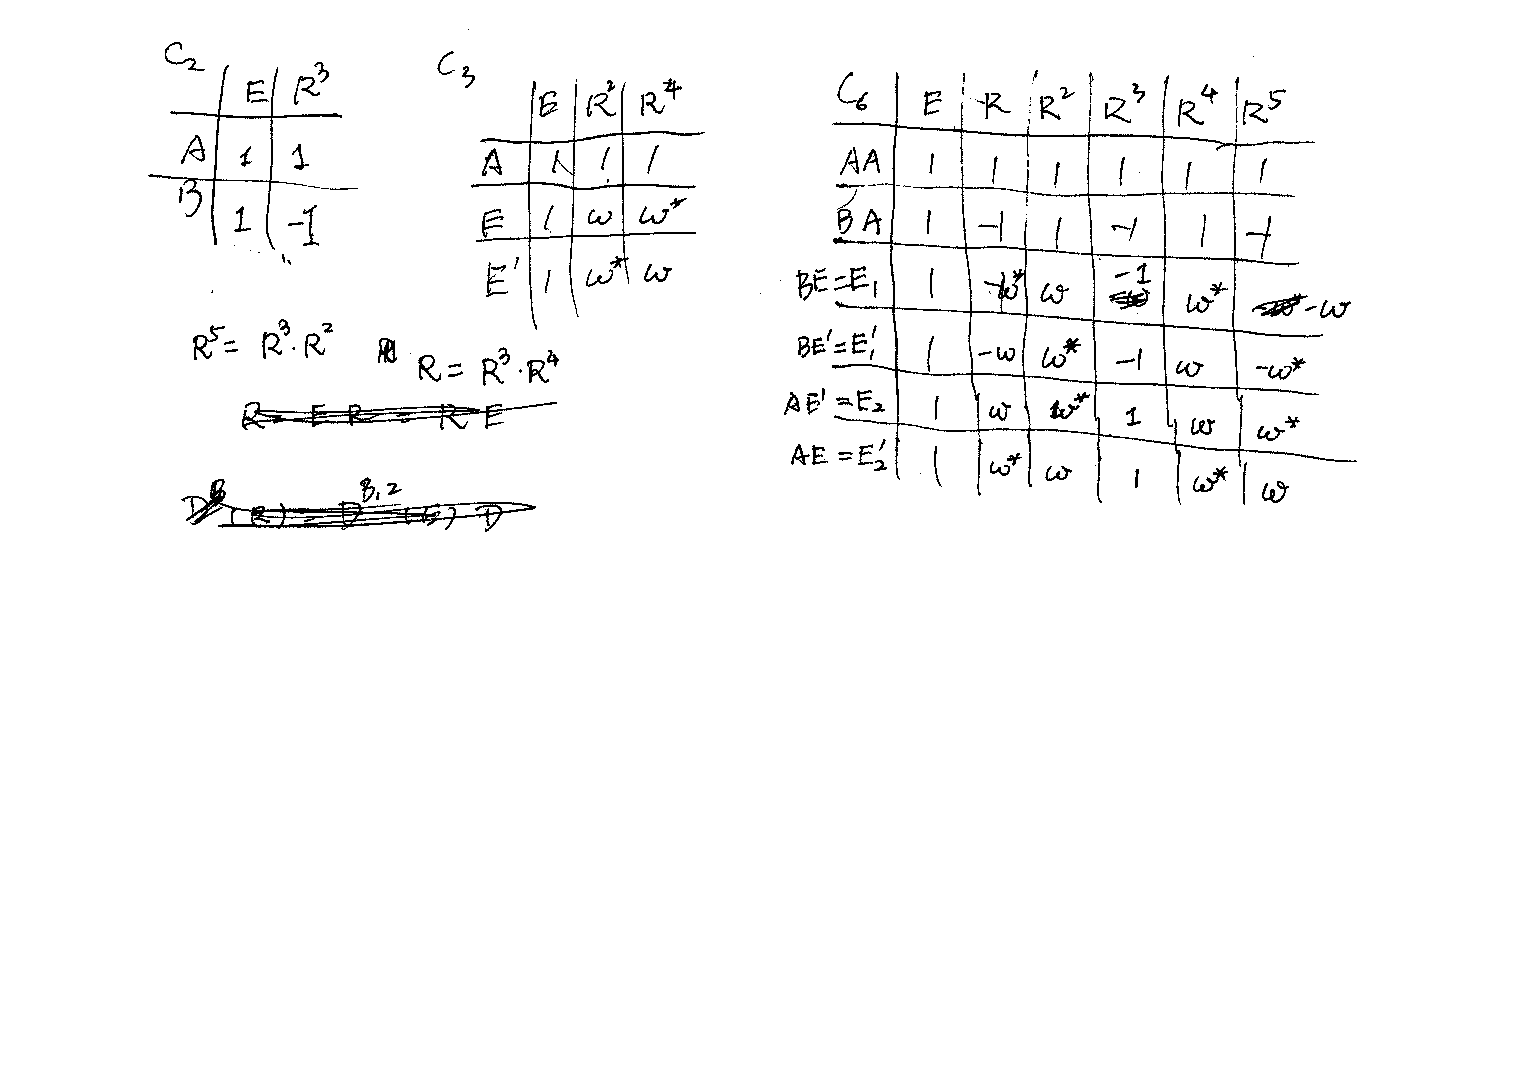
\includegraphics[width=0.8\linewidth]{scans/get-C6-character.pdf}
    \caption{Get $C_6$ Character table}
\end{figure}
\subsection{Dihedral Group \texorpdfstring{$D_n$}{}}
\label{sec:Dihedral-Group}
\begin{defi}[Dihedral Group $D_n$]
\nomenclature{Dihedral Group $D_n$}{\nomrefpage.}
    Dihedral group $D_n$ is the symmetric group of regular $n$-gons
    for $n\geq 3$. For $n=1/2$, it is usually not defined. I found that
    in book \cite{book}, $D_2$ is isomorphic to Klein Group, $D_1$ is
    of course the trivial group.
\end{defi}

But we can have another more mathematical definition of Dihedral
group. To introduce that definition, let me first explain some facts
and discuss a little bit about its conjugacy classes.

There is some important difference between the case when $n$ is odd
and when $n$ is even. When $n$ is odd, the $2$-fold axis are all
linked with the vortices of the $n$-polygon. On the contrary, when $n$
is even, there is two different $2$-fold axis. The first $n/2$
$2$-fold axises are those linked with the vortices, the second $n/2$
$2$-fold axises are those cutting through the opposite edges. 

\subsubsection{Conjugacy Classes}
Note that by fact \ref{fact:20161010-srs} one can see that such
difference mentioned will make the two classes of $2$-fold axises in
even $n$ each form their own conjugacy class. On the contrary, by the
same fact \ref{fact:20161010-srs} one sees that when $n$ is odd, all
the $2$-fold axises are in the same conjugacy class. Note that a
reflection is its own inverse, so in either cases ($n$ odd or even),
we have found self-conjugate classes.

The next conjugacy classes are about rotation. Denotes one $2\pi/n$
rotation around the $N$-fold axis by $T$, then by this very same fact
\ref{fact:20161010-srs}, $T$ and $T^{-1}$ lies in the same conjugacy
class, related by a reflection around a $2$-fold axis. This is obvious
a self-conjugate class. (Note that, when only $2\pi/n$ rotation is
considered, they form an abelian group and each rotation forms a
conjugacy class.) Similarly for the conjugacy class $\{T^m, T^{-m}\}$,
where $m$ is an integer.

In summary, this discussion shows that the conjugacy classes (all are
self-conjugate) in $D_n$
are:
\begin{fact}
    When $n$ is odd (Let $n=2n'+1$): The identity class, the class of
    all $2$-fold axis. The class of $\{ T^m, T^{-m}\}$, where
    $m=1,2,\cdots, n'$. (Why $m\leq n'$? Think about the case when
    $n=5,n'=2$.). In total $n'+2=\frac{n+3}{2}$ conjugacy
    classes/irreducible representations. All conjugacy classes are
    self-conjugate.
\end{fact}
\begin{fact}
    When $n$ is even (Let $n=2n'$): The identity class, the two
    classes of all $2$-fold axis, as discussed above. The class of
    $\{ T^m, T^{-m}\}$, where $m=1,2,\cdots, n'$. In total
    $n'+3=\frac{n+6}{2}$. All conjugacy classes are self-conjugate.
\end{fact}

\subsubsection{Formal definition of \texorpdfstring{$D_n$}{}}

Having discussed about conjugacy classes, one sees that $D_n$ can be
defined by generators.  Clearly, when $n$ is odd, $D_n$ is generated
by one rotation $2\pi/n$ and one reflection (denoted $C'_2$ in the
book \cite{book}). When $n$ is even, one might thinks that we have
three generators, i.e. the rotation by $2\pi/n$, one reflection about
vortex $C'_2$, and one reflection about middle of edges $C''_2$. But
actually it only needs two. The reflection about middle of edges can
be produced by the rotation and the reflection about vortex, or vice
versa. See this note for example:

\begin{figure}[H]
    \centering
    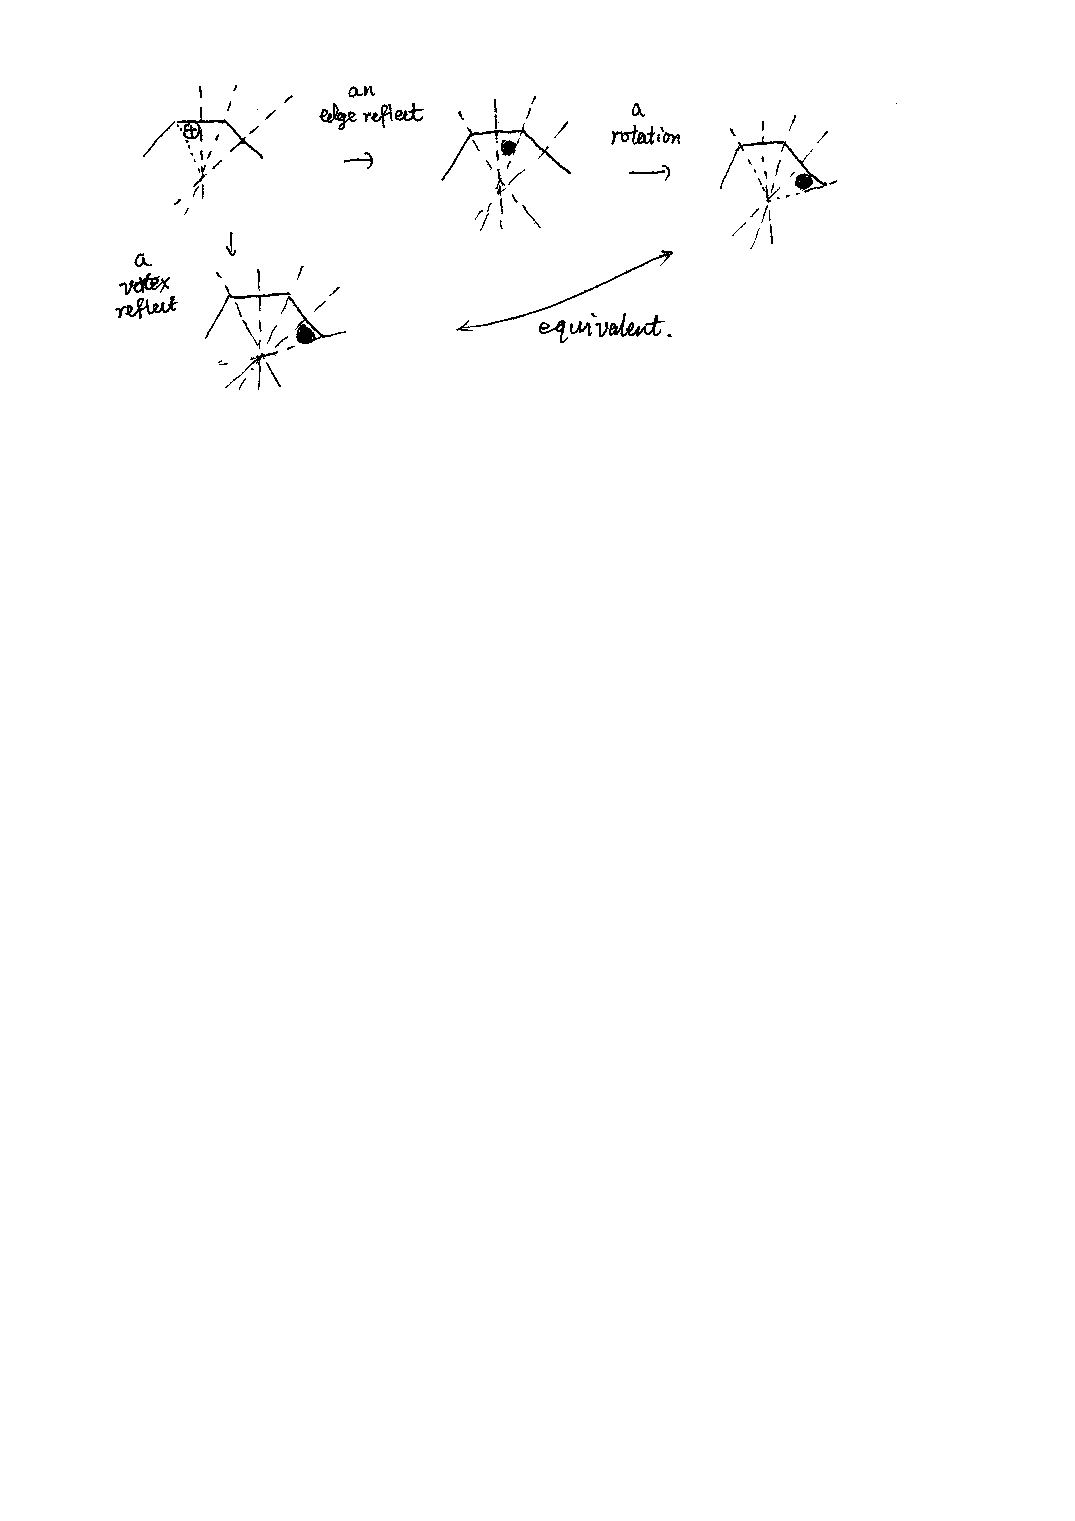
\includegraphics[width=0.8\linewidth]{scans/relate-edge-vortex.pdf}
    \caption{relate-edge-Vortex}
\end{figure}
So all in all, $D_n$ can be generated by just two elements. They are:
\begin{fact}
\label{fact:point-group-formal-def-dn}
\begin{align}
    D_n &\equiv \braket{R,S|R^n=1,S^2=1,SRS^{-1}=R^{-1}} \\
        &\equiv \braket{R,S|R^n=1,S^2=1,(SR)^2=1}
\end{align}
Here the first line symbolizes that rotation $R$ and $R^{-1}$ are in
the same conjugacy class. The second is more beautiful and symbolizes
that a roto-reflection is idempotent.
\end{fact}

Observe that by this definition, it's easy to prove that
\begin{align}
    SR &= R^{-1}S \\
    SR^{-1} &= RS
\end{align}
which are all physically intuitive. A more sophisticated law is
also physically easy to see
\begin{fact}
    \begin{equation}
        S_m R^n = R^{-n}S_m
    \end{equation}
\end{fact}
But I here give a mathematical derivation of the above formula:
\begin{proof}
    Assume $n$ is add.

    Pick a reference point in the $n$-polygon, label its vortex as $0$. Then
    let $S_0= S$ be the reflection about this vortex axis. Then label
    all the remaining vortex $2$-fold axises in the same direction as
    $R$ as $1,2,\cdots,n-1$. Obviously we have:
    \begin{align}
        S_1 &= RS_0 R^{-1} = RSR^{-1} \nonumber\\
        S_2 &= RS_1 R^{-1} = R^2 S R^{-2} \nonumber\\
        \cdots & \nonumber \\
        S_{m} &= R^{m} S R^{m}
    \end{align}
    where $m=1,2,\cdots,n-1$. Then
    \begin{align*}
        S_m R^n &= R^m S R^{-m} R^n \\
          &= R^m S R^n R^{-m}\\
          &= R^m R^{-n} S R^{-m} \\
          &= R^{-n} S_m
    \end{align*}

    When $n$ is odd, the proof is the same, except that now $S_{2m}$ is a
    vortex reflection, and $S_{2m+1}$ is an edge reflection
    ($m=0,1,\cdots (n/2-1)$). Notice that $S_1= RS_0 = RS$, we easily
    see
    \begin{align}
        S_{2m} &= R^m S R^{-m} \\
        S_{2m+1} &= R^{m+1} S R^{-m}
    \end{align}
    and the rest of the proof is the same.
\end{proof}

\subsubsection{Invariant Subgroups} (\textbf{pp.30 of \cite{book}})
By the distinction between edge and vortices type of $2$-fold axises
discussed before, one can see that there is difference in invariant
subgroup when $n$ is odd or even. For example, when $n=5$ is odd,
$D_5$ has only $C_5$ as a notrivial subgroup. But when
$n=6$ is even, it has $C_6$ (then $C_2$ and $C_3$), two copies of
$D_3$ (each formed by edge and vortex type of $2$-fold axis).

More generally, there importnat subgroup of index for $D_n$. When $n$
is odd (let $n'2n'+1$), there are one subgroup of index $2$, i.e.
$C_n'$. When $n$ is even (let $n'=n/2$), there are three invariant
subgroup of index $2$: $C_n'$, $D_n$, and $D_n'$. Denote $n$ $2$-fold
axis as $S_j$, rotation around $n$-fold axis by $2\pi/n$ as $T$,
then:
\begin{align}
    D_n &= \{E, T^2,T^4,\cdots,T^{2n-2},S_0,S_2,\cdots,S_{2n-2}\} \\
    D_n' &= \{E, T^2,T^4,\cdots,T^{2n-2},S_1,S_3,\cdots,S_{2n-1}\}
\end{align}
Note that this list is not complete. For example, $D_6$ contains other
nontrivial invariant subgroups, listed in page 30 of \cite{book}.

\subsubsection{Character Table} (\textbf{pp.66 of \cite{book}})

For $D_2$, it is isomorphic to the group
$\{1,\sigma,\tau,\sigma\tau\}$, where $\sigma$ is spatial inversion,
$\tau$ is time-reversal. Notice that this group is abelian, so it
obvious has $4$ irreducible representations. It is easy to get its
character table, which may be found on page 66, table 3.6 of
\cite{book}.

For $D_3$, it is non-abelian. As discussed previously, it has $3$
conjugacy classes, so it has 3 irreducible representations. Notice
that $D_3/C_3 \cong C_2$, so it inherets the two simple irreducible
representations of $C_2$. This gives two lines in the character
table. Also, $6-1^2-1^2=2^2$, so we have one $2$-dimensional
irreducible representation left.  Next, by fact
\ref{fact:character-of-identity}, we can determine one element in the
character for $2$-dimensional irreducible representation. The rest two
empty blanks can be filled using the orthogonal relations for the
character table.
\begin{figure}[H]
    \centering
    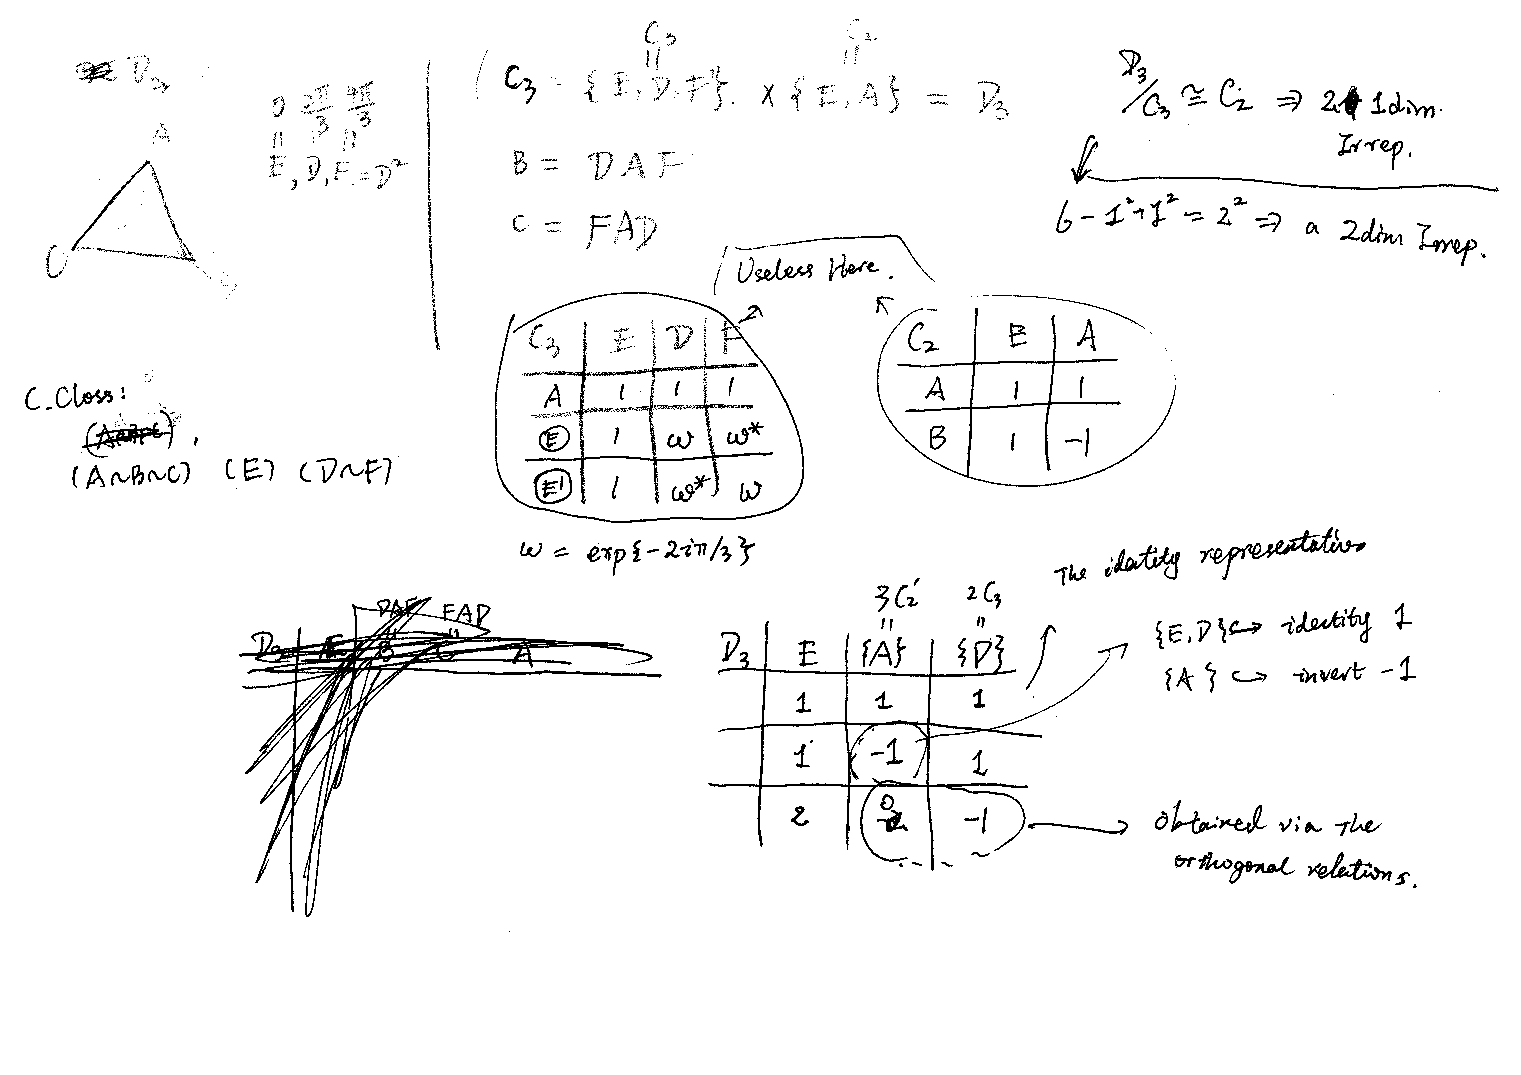
\includegraphics[width=0.8\linewidth]{scans/get-D3-character.pdf}
    \caption{Get $D_3$ Character table}
\end{figure}

For general $D_n$, see the part for irreducible representations.

\subsubsection{Irreducible representation} 

(\textbf{pp.71-74 of \cite{book}}) 

The general procedure is to use the invariant subgroup of index $2$
mentioned above to get the $1$-dimensional representations. And use
the relation $\sum_j m_j^2 = |D_n|$ and $\sum_j 1 = $ number of
conjugacy class to get the dimensional of remaining irreducible
representations. Finally use subgroup $C_n$ to construct those
representations (induced representation) and reduce these into
irreducible ones. But how to reduce them into irreducible one is
actually the most difficult part, in my opinion.

I present only vague discussion below. For details, please to ...
actually I don't know which book. The textbook \cite{book} is too
concise. Perhaps I should find some more detailed books.
% TODO Add better books.

For odd $n$, let $n=2n'+1$. We have:
\begin{align}
    \sum_{j=1}{n'+2} m_j^2 = 4n'+2
\end{align}

There is two $1$-dimensional irreducible representations, formed using
the invariant subgroup $C_{2n'+1}$. Since $4n'+2 = 2^2 n'+2$, one
guesses\footnote{Actually, the remaing ones can satisfy our condition
    only if they are $2$-dimensional. A $1$-dimensional would means an
    additional invarian subgroup of index $2$, which is not true. A
    $3$-dimensional would demand an additional $1$-dimensional
    representation to balance and get a even number. So
$2$-dimensional is the only possibility.}, that the remaining ones are
$n$ $2$-dimensional irreducible representations. They are constructed
(construction process could be found in \cite{book}) to be (notice
$D_{2n'+1}$ is generated by $T_{2n'+1}$, the rotation
$2\pi/(2n'+1)$, and $C'_2$, any one of the $2$-fold reflection):
\begin{align}
    \bar{D}^{E_j}(C_{n}) &=\left( \begin{array}{cc}
    \cos(\frac{2j\pi}{n}) & -\sin(\frac{2j\pi}{n}) \\
    \sin(\frac{2j\pi}{n}) & \cos(\frac{2j\pi}{n}) \\
        \end{array} \right) \\
    \bar{D}^{E_j}(C'_{2}) &= \left( \begin{array}{cc}
                 1 & 0 \\
                 0 & -1 \\ 
                 \end{array} \right)
\end{align}
where $j=1,2,\cdots,n$.

The case for even $n$ is simialr (let $n'=n/2$). Except that now it
has three invariant subgroup of index $2$ (see dicusson about invariant
subgroup above). So it has $2+2+2-2=4$ $1$-dimensional irreducible
representations ($-2$ for the repeated identity representation), and
$n'-1$ $2$-dimensional irreducible representations.
(we have $\sum_{j=1}^{n'+3}m_j^2 = 4n' = (n-1)2^2 + 4\cdot 1$.)
The result is exactly the same as in the the add $n$ case, and this is
why I did not write $2n'+1$ but use $n$ in the above equations.


\subsection{T-group}

\nomen{$T$ group} is the group of the symmetry of tetrahedrons. It is
a subgroup of $O$, the symmetry of cubic or octahedron (will % TODO ).

A graph is provided in the page 33 of \cite{book}.  Part of this work
has been done in the mid-term exam and is not repreated here.

The conjugacy classes:
$\{E\}$ and $\{3C_2\}$, $\{4C'_2\}$, $\{4C'^2_2\}$.

\paragraph{Character Table}
It has a subgroup of $D_2$, which can be seen from analysing the
number of elments in conjugacy classes. $D_2$ is just $C_3$ discussed
before, and it has three 1D representations. So first three line of
the character is simple to get.

The remaing representation is $3$-dimensional, so we can again fill
one element of the character table. The rest can be easily filled by
the orthogonal relations.

Details on page 66 and 33 of \cite{book}.
